\chapter{Progress \& Experiments} \label{chap:prog}
So far, we have studied on CycleGAN\cite{cyclegan}, UNIT\cite{DBLP:journals/corr/LiuBK17} and SingleGAN\cite{SingleGAN} for image-to-image translation tasks. We developed two unpaired datasets to train our network. For the cartoon domain, we've collected almost 3.1K images scrapped from various movies, e.g. \textit{Pokemon}, \textit{My Neigbour Totoro} and \textit{Kiki’s Delivery}. We used flickr dataset for the real images’ domain. Images are resized to 128×128 resolution. For implementation we used PyTorch and for hardware we used Nvidia GTX 1060. We compare our results through different architectures i.e. CycleGAN\cite{cyclegan}, UNIT\cite{DBLP:journals/corr/LiuBK17} and SingleGAN\cite{SingleGAN}.\\
In some images, \textit{cycle consistency loss} was unable to preserve content representation of input image. However, UNIT\cite{DBLP:journals/corr/LiuBK17} was able to maintain content of input image in the output. Still it has some flaws, as UNIT tends to smoothen the surface of output images, where in real world surfaces are tend to be crisp and less sharpen on the edges. In SingleGAN\cite{SingleGAN}, output images colors become faded and the content is not preserved most of the time.

%First Comparison
\begin{figure}[ht]
Input \hspace{2.7cm} CycleGAN \hspace{1.8cm} UNIT \hspace{2.4cm} SingleGAN
\begin{center}
     \begin{subfigure}
    
         
\includegraphics[scale = 0.7]{pic/in/i1.png}
     \end{subfigure}
     \hspace{0.1in}
     \begin{subfigure}
         
         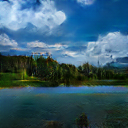
\includegraphics[scale = 0.7]{pic/cgan/c1.png}
     \end{subfigure}
     \hspace{0.1in}
     \begin{subfigure}
         
         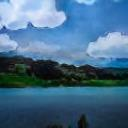
\includegraphics[scale = 0.7]{pic/unit/u1.jpg}
     \end{subfigure}
     \hspace{0.1in}
     \begin{subfigure}
        
         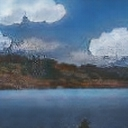
\includegraphics[scale = 0.7]{pic/sgan/s1.jpg}
     \end{subfigure}
     \begin{subfigure}
         
         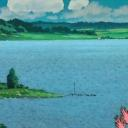
\includegraphics[scale = 0.7]{pic/in/i2.png}
     \end{subfigure}
     \hspace{0.1in}
     \begin{subfigure}
         
         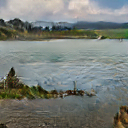
\includegraphics[scale = 0.7]{pic/cgan/c2.png}
     \end{subfigure}
     \hspace{0.1in}
     \begin{subfigure}
         
         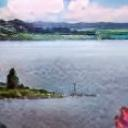
\includegraphics[scale = 0.7]{pic/unit/u2.jpg}
     \end{subfigure}
     \hspace{0.1in}
     \begin{subfigure}
        
         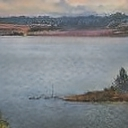
\includegraphics[scale = 0.7]{pic/sgan/s2.jpg}
     \end{subfigure}
     \begin{subfigure}
         
         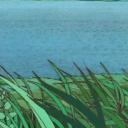
\includegraphics[scale = 0.7]{pic/in/i3.png}
     \end{subfigure}
     \hspace{0.1in}
     \begin{subfigure}
         
         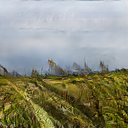
\includegraphics[scale = 0.7]{pic/cgan/c3.png}
     \end{subfigure}
     \hspace{0.1in}
     \begin{subfigure}
         
         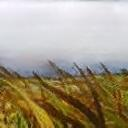
\includegraphics[scale = 0.7]{pic/unit/u3.jpg}
     \end{subfigure}
     \hspace{0.1in}
     \begin{subfigure}
        
         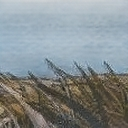
\includegraphics[scale = 0.7]{pic/sgan/s3.jpg}
     \end{subfigure}
     \begin{subfigure}
         
         
\includegraphics[scale = 0.7]{pic/in/i4.png}
     \end{subfigure}
     \hspace{0.1in}
     \begin{subfigure}
         
         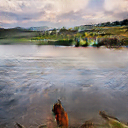
\includegraphics[scale = 0.7]{pic/cgan/c4.png}
     \end{subfigure}
     \hspace{0.1in}
     \begin{subfigure}
         
         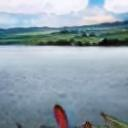
\includegraphics[scale = 0.7]{pic/unit/u4.jpg}
     \end{subfigure}
     \hspace{0.1in}
     \begin{subfigure}
        
         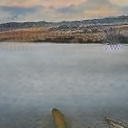
\includegraphics[scale = 0.7]{pic/sgan/s4.jpg}
     \end{subfigure}
     \begin{subfigure}
         
         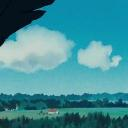
\includegraphics[scale = 0.7]{pic/in/i5.png}
     \end{subfigure}
     \hspace{0.1in}
     \begin{subfigure}
         
         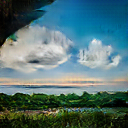
\includegraphics[scale = 0.7]{pic/cgan/c5.png}
     \end{subfigure}
     \hspace{0.1in}
     \begin{subfigure}
         
         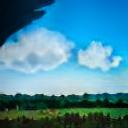
\includegraphics[scale = 0.7]{pic/unit/u5.jpg}
     \end{subfigure}
     \hspace{0.1in}
     \begin{subfigure}
        
         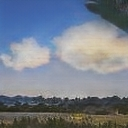
\includegraphics[scale = 0.7]{pic/sgan/s5.jpg}
     \end{subfigure}
     \begin{subfigure}
         
         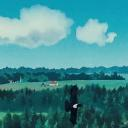
\includegraphics[scale = 0.7]{pic/in/i6.png}
     \end{subfigure}
     \hspace{0.1in}
     \begin{subfigure}
         
         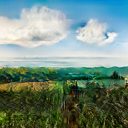
\includegraphics[scale = 0.7]{pic/cgan/c6.png}
     \end{subfigure}
     \hspace{0.1in}
     \begin{subfigure}
         
         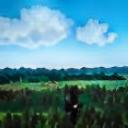
\includegraphics[scale = 0.7]{pic/unit/u6.jpg}
     \end{subfigure}
     \hspace{0.1in}
     \begin{subfigure}
        
         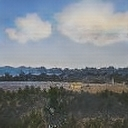
\includegraphics[scale = 0.7]{pic/sgan/s6.jpg}
     \end{subfigure}
     
     \caption{Comparison Between CycleGAN, UNIT and SingleGAN}
     \label{fig:compare1}
\end{center}
\end{figure}

%Second Comparison
\begin{figure}[ht]
Input \hspace{2.7cm} CycleGAN \hspace{1.8cm} UNIT \hspace{2.4cm} SingleGAN
\begin{center}
     \begin{subfigure}
    
         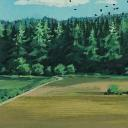
\includegraphics[scale = 0.7]{pic/in/i7.png}
     \end{subfigure}
     \hspace{0.1in}
     \begin{subfigure}
         
         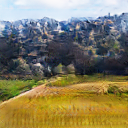
\includegraphics[scale = 0.7]{pic/cgan/c7.png}
     \end{subfigure}
     \hspace{0.1in}
     \begin{subfigure}
         
         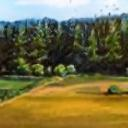
\includegraphics[scale = 0.7]{pic/unit/u7.jpg}
     \end{subfigure}
     \hspace{0.1in}
     \begin{subfigure}
        
         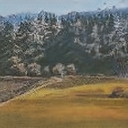
\includegraphics[scale = 0.7]{pic/sgan/s7.jpg}
     \end{subfigure}
     \begin{subfigure}
         
         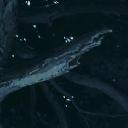
\includegraphics[scale = 0.7]{pic/in/i8.png}
     \end{subfigure}
     \hspace{0.1in}
     \begin{subfigure}
         
         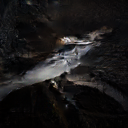
\includegraphics[scale = 0.7]{pic/cgan/c8.png}
     \end{subfigure}
     \hspace{0.1in}
     \begin{subfigure}
         
         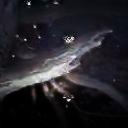
\includegraphics[scale = 0.7]{pic/unit/u8.jpg}
     \end{subfigure}
     \hspace{0.1in}
     \begin{subfigure}
        
         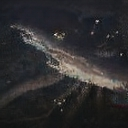
\includegraphics[scale = 0.7]{pic/sgan/s8.jpg}
     \end{subfigure}
     \begin{subfigure}
         
         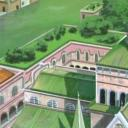
\includegraphics[scale = 0.7]{pic/in/i9.png}
     \end{subfigure}
     \hspace{0.1in}
     \begin{subfigure}
         
         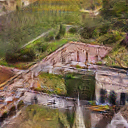
\includegraphics[scale = 0.7]{pic/cgan/c9.png}
     \end{subfigure}
     \hspace{0.1in}
     \begin{subfigure}
         
         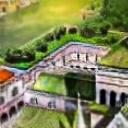
\includegraphics[scale = 0.7]{pic/unit/u9.jpg}
     \end{subfigure}
     \hspace{0.1in}
     \begin{subfigure}
        
         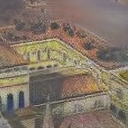
\includegraphics[scale = 0.7]{pic/sgan/s9.jpg}
     \end{subfigure}
     \begin{subfigure}
         
         
\includegraphics[scale = 0.7]{pic/in/i10.png}
     \end{subfigure}
     \hspace{0.1in}
     \begin{subfigure}
         
         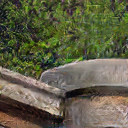
\includegraphics[scale = 0.7]{pic/cgan/c10.png}
     \end{subfigure}
     \hspace{0.1in}
     \begin{subfigure}
         
         
\includegraphics[scale = 0.7]{pic/unit/u10.jpg}
     \end{subfigure}
     \hspace{0.1in}
     \begin{subfigure}
        
         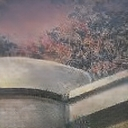
\includegraphics[scale = 0.7]{pic/sgan/s10.jpg}
     \end{subfigure}
     \begin{subfigure}
         
         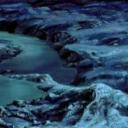
\includegraphics[scale = 0.7]{pic/in/i11.png}
     \end{subfigure}
     \hspace{0.1in}
     \begin{subfigure}
         
         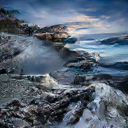
\includegraphics[scale = 0.7]{pic/cgan/c11.png}
     \end{subfigure}
     \hspace{0.1in}
     \begin{subfigure}
         
         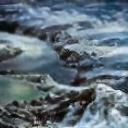
\includegraphics[scale = 0.7]{pic/unit/u11.jpg}
     \end{subfigure}
     \hspace{0.1in}
     \begin{subfigure}
        
         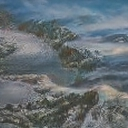
\includegraphics[scale = 0.7]{pic/sgan/s11.jpg}
     \end{subfigure}
     \begin{subfigure}
         
         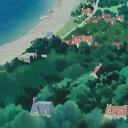
\includegraphics[scale = 0.7]{pic/in/i12.png}
     \end{subfigure}
     \hspace{0.1in}
     \begin{subfigure}
         
         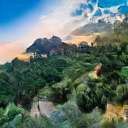
\includegraphics[scale = 0.7]{pic/cgan/c12.png}
     \end{subfigure}
     \hspace{0.1in}
     \begin{subfigure}
         
         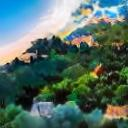
\includegraphics[scale = 0.7]{pic/unit/u12.jpg}
     \end{subfigure}
     \hspace{0.1in}
     \begin{subfigure}
        
         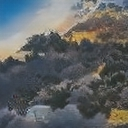
\includegraphics[scale = 0.7]{pic/sgan/s12.jpg}
     \end{subfigure}
     
     \caption{Comparison Between CycleGAN, UNIT and SingleGAN}
     \label{fig:compare2}
\end{center}
\end{figure}

%Data Flow Diagram


